\documentclass[a4paper, 12pt]{article}
\usepackage{cite}
\usepackage{multicol, caption}
\usepackage{titling}
\usepackage{graphicx}
\usepackage{tabularx}
\usepackage{subcaption}
\usepackage{url}
\newenvironment{Figure}
  {\par\medskip\noindent\minipage{\linewidth}}
{\endminipage\par\medskip}

%加這個就可以設定字體
\usepackage{fontspec}
%使用xeCJK,其他的還有CJK或是xCJK
\usepackage{xeCJK}
\usepackage[margin=0.6in]{geometry}

%字型的設定可以使用系統內的字型,而不用像以前一樣另外安裝
\setCJKmainfont{DFKai-SB}
\author{}    
\newcommand*{\citenumfont}{}

% Reducing Distance of title and date
\setlength{\droptitle}{-2cm}
\title{\textbf{Offensive Tweet Classification}}
\renewcommand\maketitlehookc{\vspace{-3.5em}}


\begin{document}
    \maketitle     
    \begin{center}
        \begin{tabular}{ccc}
            陳君彥, b04703091 & 陳柔安, b04701232 & 蕭法宣, b04705007 \\
            b04703091@ntu.edu.tw &
            b04701232@ntu.edu.tw &
            b04705007@ntu.edu.tw
        \end{tabular}
    \end{center}

    \section*{Division of Work}
        陳君彥, b04703091: 
        \begin{itemize}
            \item Generation and testing of TFIDF-Vectorized models.
            \item Generation and testing of domain knowledge based features.
            \item Creation of written report.
        \end{itemize}
        陳柔安, b04701232:
        \begin{itemize}
            \item Generation and testing of bi-LSTM.
            \item Generation and testing of CNN models.
        \end{itemize}
        蕭法宣, b04705007:
        \begin{itemize}
            \item Generation and testing of BERT model.
            \item Generation and testing of string based features.
        \end{itemize}

    \section{Introduction}
        The goal of OffensEval competition on codalab by SemEval 2019 \cite{offens} is to tag a series of tweets with regards to their offensive nature. The competition is separated into 3 subtasks.
        \begin{itemize}
            \item Subtask a: Tag a tweet based on whether the tweet is considered "offensive" or not. Tags include "OFF" and "NOT"
            \item Subtask b: If a tweet is tagged as offensive in subtask a, further tag the tweet on whether it is offensive in a targetted entity, or not targetted. Tags include "TIN" and "UNT".
            \item Subtask c: If a tweet is tagged as targetted in subtask b, further tag the tweet on whether it is targetted towards an individual, towards a group, or towards something else. Tags include "IND", "GRP", and "OTH".
        \end{itemize}

        \subsection{Dataset Analysis}
        
        \begin{center}
            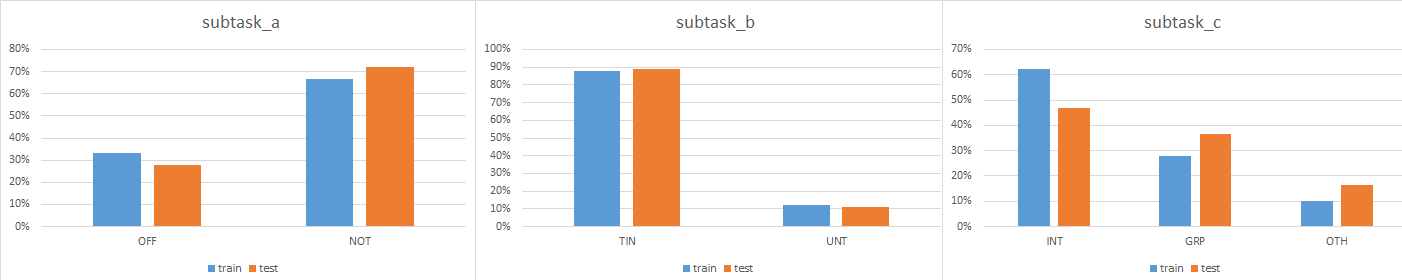
\includegraphics[width=\linewidth]{images/dist.png}
            \captionof{figure}{The percentage of each tag in the data set}
            \label{dist}
        \end{center}

        Our training dataset consists of 13240, 4400,  3876 tweets for subtask a, b, c respectively, and the testing set has 620, 240, 213 respectively. We suspect the small size in the training data, coupled with the large disparity between the tag distribution as seen in Figure \ref{dist}, contributes greatly to the difficulty in creating an accurate prediction model.
        
        \newpage
    \begin{multicols}{2}

    \section{Preprocessing}
        \subsection{Basic Text Preprocessing}
            We implemented the most common methods of text preprocessing, including the removal of stopwords, word tokenization, stemming, and lemmatizing. This was all done with the nltk package \cite{NLTK}, using the punkt corpus for stopwords, Lancaster model for stemming, and WordNet model for lemmatizing.
        \subsection{Additional processing}
            We also experimented with different additional processing that is more tailored to our tweet based data, including testing between cased and uncased text, the inclusion or removal of "tweet tags" (@USER) and twitter hashtags.

    \section{Methods}
        \subsection{Domain based features}
            \subsubsection{Subtask a}
                We considered what constituted as an "offensive" tweet to the general public, and decided that the main criteria would likely be the inclusion of the use of profanity. We downloaded a list of common profanity words that Google uses as a filter list \cite{profane}, and matched it in our tweets. 

                This method provides a very good baseline and close to our top performing models, all while being almost instanteous. We surmise that the use of a filter list is likely one of the most cost efficient ways to detect offensive languages.
            \subsubsection{Subtask c}
                We considered what it meant be be targetted towards a group, person, or issue, and arrived at the conclusion that if a tweet considered a noun that referenced a group or person, it is likely that it is targetted towards said entity, and if no such noun was found, it was non towards an entity in particular. 

                This idea was implemented through the use of "Named Entity Relationship taggers" created by Stanford \cite{stanNER}, as well as the SpaCy \cite{spacy2} tagger. This performed much less poorly than our more advanced models, but still provided a baseline that can be trained and predicted on the fly.
        \subsection{General Classification Models}
            We also tried to take a general approach to this classfication problem, as it relies somewhat less on specific natural language characteristics, and more on just pattern recognition. After preoprocessing, we transformed the tweets into vectors using TFIDF-Vectorizers, and ran the 3 subtasks through Naive Bayes, K-Nearest Neighbours, Decision Tree, Random Forest, and Linear Regression, all using the provided models found in the Sci-kit Learn \cite{scikit-learn} packages.

            Of the tested models, Decision Tree and Linear Regression performed the best, though still somewhat short of our BERT method, while Random Forest performed slightly poorer, while also requiring much longer to train.
        \subsection{BERT Models}
            We also elected to use Google's BERT \cite{bert} designed for NLP tasks. This model is the best performing method out of all of the ones we tried, but required large amounts of computation power, and a very long training time for each subtask. This leads to this method being viable for our rather small dataset, but could possibly be not worth it for larger, more complete data.
        \subsection{Neural Network Models}
            \subsubsection{CNN}
                Based on a paper from WildML \cite{wildML}, we decided to take a non traditional approach and tried out the use of CNN in our prediction. The use of CNN with natural language leads to a behaviour similar to an optimized version of n-gram models, segmenting our tweets into semantical parts. Surprisingly, the model performed quite well, similar to general machine learning models, while requiring extremely low training time.
            \subsubsection{BiLSTM}
                We tried out the BiLSTM from the Keras package \cite{keras}, which is often used in NLP modelling. However, our model performed poorly, sometimes worse than our general models, while also taking a long time to train, and we neglected to investigate further.
    \section{Experiments}
        The following are the experiments we did for each model used in our testing. Our computer ran a Intel 9400f CPU clocked at 4.1GHz x1/ 3.9GHz x6, running Windows 10 Home Edition. For all time related metrics mentioned, it can be assumed that the testing conditions were all roughly equivalent.
    \subsection{Domain Knowledge Models}
        \begin{center}
            \begin{tabular}{l|cc}
                Method & Training & Testing \\
                \hline
                Profanity Filter (a) & 0.6887 & 0.7043 \\
                SpaCy NER (c) & 0.3114 & 0.3082 \\
                Stanford NER (c) & 0.2516 & 0.2992 \\
            \end{tabular}       
            \captionof{table}{Performance of domain knowledge based models. Brackets denote subtasks.}     
            \label{domainTable}
        \end{center}

        As seen in Table \ref{domainTable}, we achieved acceptable figures using a profanity filter on subtask a. This was done by downloading a list of profanity filter words used by Google, as well as adding in some extra words manually by looking at the training dataset and noting words with a high tfidf disparity between offensive and non-offensive tweets. 
        
        Subtask C performed rather poorly however, only beating a baseline of tagging all as "IND" (0.210). As the two NER taggers we used are quite known for being rather performant, we suspect the issue is likely to be from the difficulty in labelling proper nouns, as well as the "unclean" data found by mistypes, hashtags, or slangs often found in tweets.
    \subsection{General Classification Models}
        \begin{center}
            \begin{tabular}{l|ccc}
                Method & Subtask a & Subtask b & Subtask c \\
                \hline
                MNB & 0.4851 & 0.4703 & 0.2819 \\
                KNN & 0.3900 & 0.4742 & 0.3507 \\
                DT & 0.7281 & 0.5530 & 0.4396 \\
                RF & 0.7213 & 0.5045 & 0.4379 \\
                LR & 0.6982 & 0.5282 & 0.4346
            \end{tabular}       
            \captionof{table}{Performance of general machine learning models.}     
            \label{generalTable}
        \end{center}

        As seen in Table \ref{generalTable}, our decision tree, random forest, and linear regression model performed much better in subtask c, while Naive-Bayes and K-Nearest Neighbours fell far short in both tasks. 
        
        While training, we noticed a large disparity between the validation accuracy for subtask b and c, somtimes upwards of 0.90 even with proper loss functions. We took a look at the dataset, and found that the training set and testing set differ substantially with regards to class imbalance as well as overall content, enough to cause our models to overfit greatly. We can see this trend continue to occur with other more sophisticated models.

        Each model took around 30 minutes to train, and didn't scale greatly with an increase in dataset size.

    \subsection{BERT}
        \begin{center}
            \begin{tabular}{l|ccc}
                Method & Subtask a & Subtask b & Subtask c \\
                \hline
            \begin{tabular}{@{}l@{}}No Preprocess \\ Uncased\end{tabular} & 0.7774 & 0.6874 & 0.5731 \\
            \begin{tabular}{@{}l@{}}No Preprocess \\ Cased\end{tabular} & 0.7734 & 0.6870 & 0.5766 \\
            \begin{tabular}{@{}l@{}}Preprocess \\ Uncased\end{tabular} & 0.7875 & 0.6868 & 0.5726 \\
            \begin{tabular}{@{}l@{}}Preprocess \\ Cased\end{tabular} & 0.8023 & 0.6827 & 0.5986
            \end{tabular}       
            \captionof{table}{Performance of BERT models}     
            \label{bertTable}
        \end{center}

        As seen in Table \ref{bertTable}, our BERT model returned the best results out of all the methods. We tested with using cased and uncased data, which gave us much better results with cased data on subtask a and c. 
        
        As most tweets are made through a phone app these days, which automatically capitalize the first letters of proper nouns, we suspect this leads a better recognition of named entities in our model, leading to a higher accuracy on subtask c.

        A major problem with BERT however, is the massive amount of time required to train the model. With our relatively small data set size, it still took 4.5 hours to train on on subtask a, and 1.5 hours on subtasks b and c, with the time proportional to data set size. With some additional tuning, it could run slightly faster, though we realize that this method may not be very useful as of now, beyond the scope of a competition with no time constraints.

        \newpage
        \subsection{Neural Network Models}
        \begin{center}
            \begin{tabular}{l|ccc}
                Dataset & Subtask a & Subtask b & Subtask c \\
                \hline
                CNN & 0.613 & 0.928 & 0.442 \\
                BiLSTM & 0.630 & 0.916 & 0.452 \\
                BiGRU & 0.602 & 0.913 & 0.436
            \end{tabular}       
            \captionof{table}{Validation Set accuracy of NN model.}
            \label{nnValidTable}
        \end{center}

        \begin{center}
            \begin{tabular}{l|ccc}
                Dataset & Subtask a & Subtask b & Subtask c \\
                \hline
                CNN & 0.738 & 0.655 & 0.472 \\
                BiLSTM & 0.702 & 0.638 & 0.435 \\
                BiGRU & 0.686 & 0.612 & 0.471
            \end{tabular}       
            \captionof{table}{Testing Set accuracy of NN model.}     
            \label{nnTestTable}
        \end{center}
        
        As seen in Table \ref{nnValidTable} and \ref{nnTestTable}, our neural network based models also perform quite well, being on par for subtask a and c, and outperforming on subtask b. Of note is the large difference between the validation and testing accuracy on subtask b, which indicates a very high degree of overfitting on our model. As mentioned before, we speculate that this is due to the large tag and data discrepency between the two data sets. The creator of the OffensEval competition mentioned in their final report that they wish to tackle these two areas in future iterations, and we hope to see a better outcome should it happen.
        \begin{center}
            \begin{tabular}{l|ccc}
                Dataset & Subtask a & Subtask b & Subtask c \\
                \hline
                CNN & 31s & 10s & 41s \\
                BiLSTM & 61s & 22s & 81s \\
                BiGRU & 56s & 17s & 81s
            \end{tabular}       
            \captionof{table}{Training time for each NN model.}     
            \label{nnTimeTable}
        \end{center}

        Table \ref{nnTimeTable} shows the training time for each of our NN models, which provides a very clear insight on the advantages that such models can provide. Compared to the 30+ minutes on general machine learning models, or hours long training on BERT, our neural networks can achieve an very acceptable rate of accuracy all while being incredibly fast to train. Coupled with the ease of performing "warm start" training on such models means that this method can be very cost effective, particularly in a online training method.
    \end{multicols}
    
    \section{Conclusion}
    In this paper, we trained NLP models to recognize offensive language in tweets, as well as additional analysis on targetation of entities. We tested a wide range of models, including basic count and filter based models, general machine learning methods, and deep learning NLP models. Our best performing model, BERT, achieve a testing accuracy of 0.8023, 0.6827, and 0.5986 on the three subtasks, which would have attained ranks 9, 11, and 10 in the original competition. However, the long training time required for BERT means that we find it hard to recommend using it in a real world scenario, and would consider the use of neural network based models like CNN should such circumstances arise.

    For possible future works, we would like to try this problem set again on a more complete data set, and perhaps do some additional tuning or leverage the power of GPUCompute to increase the performances of our models to acceptable rates. We would also like to further analyze the reason behind the overfitting issue on subtask b, and possibly come up with a solution to remedy such a problem.

        \vskip 5cm
\bibliography{report}{}
\bibliographystyle{ieeetran}

\end{document}
